\documentclass[greek]{beamer}
%\usepackage{fontspec}
\usepackage{amsmath,amsthm}
\usepackage{unicode-math}
\usepackage{xltxtra}
\usepackage{graphicx}
\usetheme{CambridgeUS}
\usecolortheme{seagull}
\usepackage{hyperref}
\usepackage{ulem}
\usepackage{xgreek}

\usepackage{pgfpages} 
\usepackage{tikz}
%\setbeameroption{show notes on second screen}
%\setbeameroption{show only notes}

\setsansfont{Calibri}

\usepackage{multicol}

\usepackage{appendixnumberbeamer}

\usepackage{polynom}

\usepackage{pgffor}

\setbeamercovered{transparent}
\beamertemplatenavigationsymbolsempty

\title{Συναρτήσεις}
\subtitle{Ακρότατα, Άρτιες - Περιττές}
\author[Λόλας]{Κωνσταντίνος. Λόλας}
\date{}

\begin{document}

\begin{frame}
      \titlepage
\end{frame}

\section{Θεωρία} 
\begin{frame}{Ακρότατα Συναρτήσεων}
      \begin{block}{Ορισμός}
            Μία συνάρτηση $f$ είναι με πεδίο ορισμού το $Α$, λέμε ότι παρουσιάζει \emph{μέγιστο} στο $x_0\in Α$ το $f(x_0)$, όταν:
            $$f(x)\le f(x_0)\text{για κάθε } x\in Α$$
            $\lim\limits_{x \to \infty}{ x+2 }$
      \end{block} \pause
      \begin{block}{Ορισμός}
            Μία συνάρτηση $f$ είναι με πεδίο ορισμού το $Α$, λέμε ότι παρουσιάζει \emph{ελάχιστο} στο $x_0\in Α$ το $f(x_0)$, όταν:
            $$f(x_0)\le f(x)\text{για κάθε } x\in Α$$
      \end{block}
\end{frame}

\begin{frame}{Ο τσομπάνης και τα πρόβατα}
      Στάνη, πλαγιά, φράχτης, πρόβατα, τσομπάνης... \pause
      \begin{alertblock}{Προσοχή}
            \begin{itemize}
                  \item Ποιό είναι το πρόβατο στο ψηλότερο σημείο?
                  \item Ποιό είναι το ψηλότερο σημείο της στάνης?
                  \item Ποιό σημείο του φράχτη...
            \end{itemize}
      \end{alertblock}
      \emph{Φράγμα(άνω/κάτω)}, \emph{sup/inf}, \emph{max/min}
\end{frame}

\begin{frame}{Quiz time Σ-Λ}
      Μια συνάρτηση:
      \begin{itemize}
            \item έχει πάντα μέγιστο\pause
            \item έχει πάντα ακρότατο\pause
            \item έχει το πολύ ένα \pause
            \item μπορεί να έχει μέγιστο και όχι ελάχιστο \pause
            \item μπορεί να έχει 3 ακριβώς ελάχιστα \pause
            \item μπορεί να έχει άπειρα
      \end{itemize}
\end{frame}

\begin{frame}{Λίγο ιστορία}
      Γνωστά ακρότατα, τυπικών συναρτήσεων:
      \begin{itemize}
            \item $f(x)=x^2$\pause, $f(x)\ge f(0)$ \pause
            \item $f(x)=αx^2+βx+γ$, $α>0$\pause, $f(x)\ge f(-\frac{β}{2α})$ \pause
            \item $f(x)=|x|$\pause, $f(x)\ge f(0)$ \pause
            \item $f(x)=x+\frac{1}{x}$, $x>0$\pause, $f(x)\ge f(1)$
            \item $f(x)=ημ(2x)$\pause, $f(x)\ge f(k\pi + \frac{\pi}{2} - \frac{\pi}{4})$ \pause, $f(x)\le f(k\pi + \frac{\pi}{4})$
      \end{itemize}
\end{frame}

\begin{frame}{Συμμετρίες...}
      \begin{block}{Ορισμός}
            Μία συνάρτηση $f$ είναι \emph{άρτια} σε ένα διάστημα $Δ$ αν για κάθε  $ x\in Δ$
            $$-x\in Δ \text{ και } f(-x)=f(x)$$
      \end{block} \pause
      \begin{block}{Ορισμός}
            Μία συνάρτηση $f$ είναι \emph{περιττή} σε ένα διάστημα $Δ$ αν για κάθε  $ x\in Δ$
            $$-x\in Δ \text{ και } f(-x)=-f(x)$$
      \end{block}
\end{frame}

\begin{frame}{Quiz Time}
      \begin{itemize}
            \item Υπάρχει τουλάχιστον μια άρτια συνάρτηση \pause
            \item Υπάρχει τουλάχιστον μία περιττή συνάρτηση \pause
            \item Υπάρχει συνάρτηση που δεν είναι άρτια ούτε περιττή
      \end{itemize}
\end{frame}

\section{Ασκήσεις}
\begin{frame}{Εξάσκηση}
      \centering
      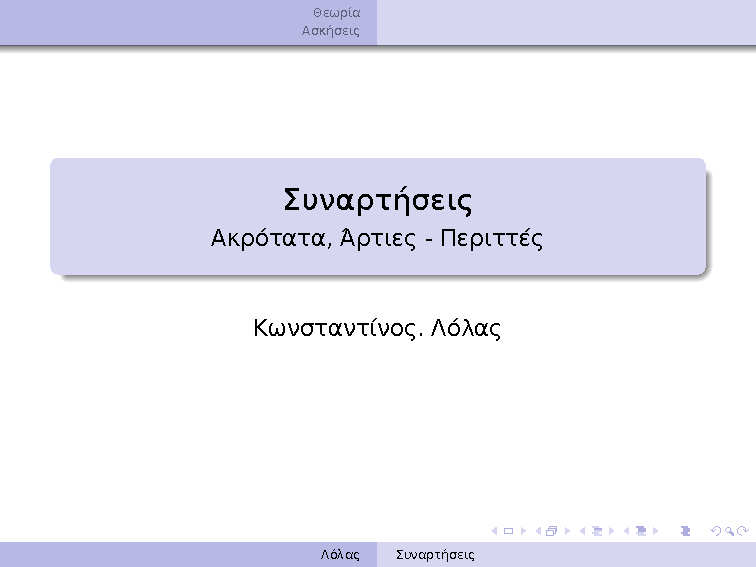
\includegraphics[width=0.35\textwidth]{"images/1.3.2 Μονοτονία.png"}

      Στο διπλανό σχήμα φαίνεται η γραφική παράσταση μιας συνάρτησης $f$
      \begin{enumerate}
            \item Να βρείτε τις θέσεις ακροτάτων και τα ακρότατα της $f$\pause
            \item Να δείξετε ότι $-1\le f(x) \le 3$ για κάθε $x\in[-2,2]$\pause
            \item Να δείξετε ότι $f(α)-f(β)\le 4$, $α$, $β\in[-2,2]$ \pause
            \item Να λύσετε
                  \begin{enumerate}
                        \item Την εξίσωση $f(x)=1$ \pause
                        \item Την ανίσωση $f(x)>-1$
                  \end{enumerate}
      \end{enumerate}
\end{frame}

\begin{frame}{Εξάσκηση}
      Να βρείτε τα ολικά ακρότατα των συναρτήσεων:
      \begin{enumerate}
            \item $|e^x-1|$ \pause
            \item $f(x)=(e^x-1)^2(x-1)^4$ \pause
            \item $f(x)=x^2-2x-5$
      \end{enumerate}
\end{frame}

\begin{frame}{Εξάσκηση}
      Δίνεται η συνάρτηση $f(x)=\frac{1}{x}$, $x>0$. Από σημείο $Μ$ της $C_f$ φέρνουμε παράλληλες ως προς τους άξονες $y'y$ και $x'x$ που τέμνουν τον $x'x$ στο $Α$ και τον $y'y$ στο $Β$. Να βρείτε τη θέση του σημείου $Μ$ για το οποίο η περίμετρος του ορθογωνίου $ΟΑΜΒ$ γίνεται ελάχιστη (όπου $Ο$ η αρχή των αξόνων).
\end{frame}

\begin{frame}{Εξάσκηση}
      Έστω $f:\mathbb{R}\to\mathbb{R}$ μία συνάρτηση, με $f(0)=1$, για την οποία ισχύει:
      $$f(x)\ge x+1 \text{, για κάθε } x\in\mathbb{R}$$
      Για κάθε $x\in\mathbb{R}$ θεωρούμε τα σημεία $Α(x,f(x))$ και $Β(f(x),x)$. Να βρείτε την ελάχιστη απόσταση των σημείων $Α$ και $Β$.
\end{frame}

\begin{frame}{Εξάσκηση}
      Έστω συνάρτηση $f:\mathbb{R}\to \mathbb{R}$ η οποία παρουσιάζει ελάχιστο μόνο στο $1$ το $2$.
      \begin{enumerate}
            \item Να δείξετε ότι $f(x)\ge 2$ για κάθε $x\in\mathbb{R}$. \pause
            \item Να λύσετε την εξίσωση $f(x)+(x-1)^2=2$ \pause
            \item Αν ισχύει $f(α)+f(\ln β)=4$, να βρείτε τις τιμές των $α$ και $β$.
      \end{enumerate}
\end{frame}

\begin{frame}{Εξάσκηση}
      Δίνεται η συνάρτηση $f(x)=\sqrt{x^2+1}$.
      \begin{enumerate}
            \item Να βρείτε το ελάχιστο της συνάρτησης $f$ και τη θέση που το παρουσιάζει \pause
            \item Να λύσετε την εξίσωση $\sqrt{x^2+1}=συνx$
      \end{enumerate}
\end{frame}

\begin{frame}{Εξάσκηση}
      Να εξετάσετε αν οι παρακάτω συναρτήσεις είναι άρτιες ή περιττές
      \begin{enumerate}
            \item $f(x)=xημ\dfrac{1}{x}$ \pause
            \item $f(x)=\ln \dfrac{1-x}{1+x}$, $x\in (-1,1)$
      \end{enumerate}
\end{frame}

\begin{frame}{Εξάσκηση}
      Έστω η συνάρτηση $f(x)=\ln (x+\sqrt{x^2+1})$
      \begin{enumerate}
            \item Να βρείτε το πεδίο ορισμού της συνάρτησης $f$ \pause
            \item Να δείξετε ότι η συνάρτηση είναι περιττή.
      \end{enumerate}
\end{frame}

\begin{frame}{Εξάσκηση}
      Έστω $f:\mathbb{R}\to\mathbb{R}$ μία συνάρτηση με $f(1)=2$ η οποία είναι γνησίως μονότονη και περιττή. Να λύσετε την ανίσωση:
      $$f(x-1)+f(x-3)<5(2-x)$$
\end{frame}

\begin{frame}{Εξάσκηση}
      Έστω $f:\mathbb{R}\to\mathbb{R}$ μία περιττή συνάρτηση, για την οποία ισχύει:
      $$(x^2+1)f(x)\le 2x \text{, για κάθε } x\in\mathbb{R}$$
      Να βρείτε:
      \begin{enumerate}
            \item το $f(0)$ \pause
            \item τον τύπο της συνάρτησης $f$
      \end{enumerate}
\end{frame}

\begin{frame}{Εξάσκηση}
      Έστω $f:\mathbb{R}\to\mathbb{R}$ μία συνάρτηση, για την οποία ισχύει
      $$f(x+y)=f(x)+f(y)\text{, για κάθε } x,y\in\mathbb{R}$$
      Να εξετάσετε αν είναι άρτια ή περιττή
\end{frame}

\begin{frame}
      Στο moodle θα βρείτε τις ασκήσεις που πρέπει να κάνετε, όπως και αυτή τη παρουσίαση
\end{frame}

\end{document}
